%
% TEXTOS SOBRE O PENSAMENTO MUSICAL
% ---------------------------------
% Agustín de Hipona (San Agustín)
%
\begin{multicols}{2}
%
%\subsection*{Pensadores e textos}\label{pensadores-textos}
%
  \paragraph{Hildegard de Bingen (1098-1179): \emph{Epístola a los prelados de Magnucia}}\label{Hildegard de Bingen}
%
  Hildegard de Bingen é un dos personaxes máis da Idade media. Foi abadesa do convento de Rupertsberg, que ela mesma fundara. As súas dedicacións foron moi diversas: era experta en botánica, medicina e outras ciencias; escribiu numerosos libros de visións proféticas que lle valeron o sobrenome de ``Sibila do Rin''; foi conselleira de papas, bispos, emperadores e reis; compuxo numerosas pezas musicais e obras teatrais con música. No seu amplo epistolario, dirixido a numerosas personalidades da súa época, trata moi diversos temas.

  A \emph{epístola aos prelados de Maguncia} xorde dunha situación concreta: este bispado, ao que pertencía o convento de Rupertsberg, prohibira á comunidade cantar o oficio, tras un conflito polo enterro en sagrado dun excomungado. A abadesa responde facendo unha contundente defensa da música.

\begin{Figura}
  \centering
  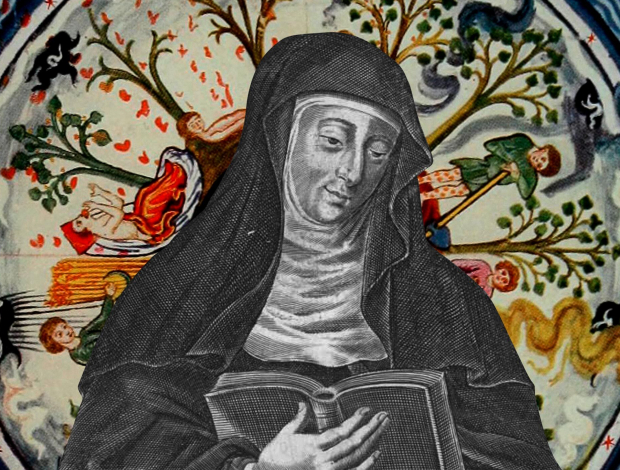
\includegraphics[width=0.75\textwidth]{ud-03/Hildegard de Bingen.jpg}
  \captionof{figure}{Hildegard de Bingen (1098-1179).\\
  (Fonte: wikimedia commons)}
  \label{fig:Hildegard-Bingen}
\end{Figura}
%
\end{multicols}
%
\vspace*{0.05cm}
\begin{quote}
\small{
Y vi algo más —pues en obediencia vuestra hemos dejado de cantar el Divino Oficio, celebrándolo solo con la lectura en silencio— y oí una voz que venía de la luz viva, hablando de las diversas formas de alabanza de las que habla David en los Salmos: «Alabadlo con el sonido de la trompeta, alabadlo con el salterio y la cítara, alabadlo con el tímpano y el coro, alabadlo con las cuerdas y el órgano, alabadlo con los sonoros címbalos, alabadlo con los címbalos del júbilo. Que todo espíritu alabe al Señor». [...] Cuando nos esforzamos seriamente en alabarlo, rememoramos cómo buscó el hombre la voz del Espíritu vivo, que Adán perdió por su desobediencia [...] Pues Adán perdió esa semejanza con la voz angélica que tuvo en el Paraíso, y así se durmió esa ciencia musical de que estaba dotado antes de su pecado. Pero Dios, que repone las almas de los elegidos en su estado original de felicidad por la luz de la verdad, forjó en su sabiduría esto: que cuando el Espíritu, con una infusión profética, renovara el corazón de muchos, recobraran estos por esta iluminación interior todo lo perdido de lo que poseía Adán antes del castigo.

Y para que la humanidad, más que rememorar el destierro de Adán, fuera despertada también a estas cosas —la divina dulzura y la alabanza que había disfrutado Adán antes de su caída—, los mismos profetas, enseñados por el Espíritu que habían recibido, no solo compusieron salmos y cánticos, que se cantarían para encender la devoción de quienes los oyeran, sino que también inventaron diversos instrumentos del arte musical, que serían tocados con gran variedad de sonidos. Lo hicieron para que los oyentes, tanto por el sonido de estos instrumentos como por el sentido de las palabras cantadas con su acompañamiento, fuesen educados en asuntos del interior, impulsados y espoleados por objetos exteriores. Hombres sabios y aplicados imitaron a estos santos profetas e inventaron numerosos tipos de instrumentos humanos, de modo que pudieran hacer música para el deleite de sus almas y adaptar lo que cantaban con las pulsaciones de sus dedos, como rememorando que Adán fue formado por el dedo de Dios (que es el Espíritu Santo); ese Adán en cuya voz, antes de su caída, residía el sonido de toda armonía y la dulzura de todo el arte musical; y si hubiera permanecido en el estado en que fue creado, la fragilidad de los hombres mortales no podrían soportar la potencia y sonoridad de su voz. [...]

Por tanto, quienes sin una razón segura y de peso imponen silencio en la iglesia en materia de cantos de alabanza a Dios, y privan así injustamente a Dios de su alabanza en la tierra, serán asimismo privados de la participación en las alabanzas angélicas que se oyen en el Cielo, salvo que hagan reparación por arrepentimiento sincero y penitencia humilde.
}
\end{quote}
%
\begin{ejercicio}[Pensamento musical Idade Media]
  \begin{enumerate}[1.-]
  \item
    En que época das que coñeces da Idade Media sitúas cronolóxicamente a autora do anterior texto? \ldots
%    \vspace*{0.5cm}
  \item
    Sinala no texto aquelas palabras que destacarías sobre a concepción da música da autora. \\
    \vspace*{8.10cm}
  \end{enumerate}
\end{ejercicio}
